\documentclass[tikz]{standalone}
\usepackage{fontspec}
\renewcommand*{\familydefault}{\sfdefault}
\usepackage{standalone}
\usetikzlibrary{arrows.meta, decorations.pathreplacing, shapes.geometric}
\usetikzlibrary{bayesnet}

\begin{document}

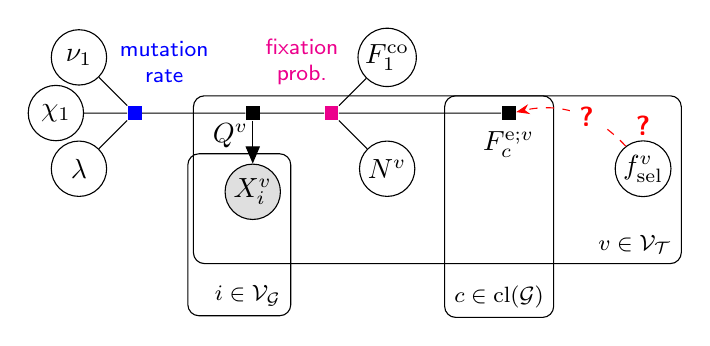
\begin{tikzpicture}

% Define nodes
\path (0,0)
node[obs] (X) {\(X^v_i\)}
(X) +(-0.7,-1) coordinate (site)
(X) +(90:1.0 cm) node[factor] (Q) {}
(Q) +(0:1.0 cm) node[factor, magenta] (fix) {}
(Q) +(-135:0.4 cm) node (Q2) {\(Q^v\)}
(fix) +(-45:1.0 cm) node[latent] (N) {\(N^v\)}
(fix) +(0:2.25 cm) node[factor] (Fc) {}
(fix) +(45:1.0 cm) node[latent] (Fco) {\(F_1^\mathrm{co}\)}
(Fc) +(0:1.75 cm) coordinate (tree)
(Fc) +(-90:0.4 cm) node (Fc2) {\(F_c^{\mathrm{e};v}\)}
(Fc) +(0:1.25 cm) coordinate (F)
(Q) +(180:1.5 cm) node[factor, blue] (mut) {}
(mut) +(180:1.0 cm) node[latent] (chi) {\(\chi_1\)}
(mut) +(-135:1.0 cm) node[latent] (lambda) {\(\lambda\)}
(mut) +(135:1.0 cm) node[latent] (nu) {\(\nu_1\)}
(site -| Fc) coordinate (clique)
;

\draw[->] (Q) -- (X);
\draw
(Q) -- (fix)
(Fc) -- (fix)
(Fco) -- (fix)
(N) -- (fix)
(mut) -- (Q)
(mut) -- (lambda)
(mut) -- (chi)
(mut) -- (nu)
;

\path[] (Fc) to[out=90,in=90] coordinate[near start] (FcF) (F);
\path (Fc) ++(0:1.0 cm) +(-45:1.0 cm) node[latent] (fsel) {\(f^v_\mathrm{sel}\)};

% Plates
\plate {Xtree} {(X) (Q2) (N) (Fc) (fsel) (tree)} {\(v\in\mathcal{V}_\mathcal{T}\)} ;
\plate {Xsite} {(X) (site)} {\(i\in\mathcal{V}_\mathcal{G}\)} ;
\plate {Xclique} {(Fc) (Fc2) (clique) } {\(c\in\mathrm{cl}(\mathcal{G})\)} ;

\begin{scope}[font=\bfseries, pos=0.4, text=red]
\draw[dashed, red, -Stealth] (fsel) to[bend right] node[pos=0.4, fill=white] {?} (Fc);
\path[anchor=south] (fsel) +(90:0.3 cm) node {?} ;
\end{scope}

\path
(mut) +(60:0.75 cm) node[font=\footnotesize, blue, align=center] {mutation \\ rate}
(fix) +(120:0.75 cm) node[font=\footnotesize, magenta, align=center] {fixation \\
prob.}
;

\end{tikzpicture}

\end{document}
